\chapter{烯醇、烯醇负离子与羟醛反应}\label{ch:b2:enolates-aldol}

每当细胞分解葡萄糖时，一种酶会把一个六碳糖
磷酸酯裂解为两个三碳片段，即逆向进行的羟醛反应。正向进行时，
同一反应可把两个羰基化合物连接成一个，
这是化学家构建碳–碳键最常用的方法。它依赖于一项
前几章只略有涉及的性质：与羰基相邻的
氢原子具有酸性，移去其中一个，使羰基旁的碳
成为亲核试剂。

\begin{recall}
本科一年级分册：$\mathrm pK_a$ 与主反应、碳负离子、动力学控制与
热力学控制、羰基的亲核加成、E1 与 E2 消除、炔烃的
水合（烯醇发生重排）。\Cref{ch:b2:frontier-orbitals}：两可亲核试剂。
\Cref{ch:b2:acyl-substitution}：酯与酰基取代。
\end{recall}

\section{酮–烯醇互变异构}

\begin{definition}[互变异构]\label{def:b2:enolates-aldol:tautomerism}
\emph{互变异构体}\index{互变异构体}是通过移动一个氢原子和一个
双键而相互转化的同分异构体。在\emph{酮–烯醇互变异构}\index{酮–烯醇互变异构}中，
羰基旁碳上带一个氢的羰基化合物（酮式）与其
\emph{烯醇}\index{烯醇}处于平衡，它是含 \ce{C=C} 双键的醇。
\end{definition}

\begin{omfigure}
\setchemfig{atom sep=2em}
\schemestart
\chemfig{H_3C-C(=[2]O)-CH_3}
\arrow{<=>[\ce{H+} 或 \ce{HO-}][催化]}[,2.2]
\chemfig{H_3C-C(-[2]OH)=CH_2}
\schemestop
\par\vspace{6pt}

{\small 丙酮及其烯醇，即丙-1-烯-2-醇。酸（羰基氧质子化，随后失去
一个 $\alpha$ 氢）或碱（夺去一个 $\alpha$ 氢，随后使氧质子化）
催化该互变；平衡强烈偏向酮式一侧。}
\end{omfigure}

\begin{proposition}[烯醇含量]\label{prop:b2:enolates-aldol:enol-content}
简单醛和酮只含痕量烯醇；1,3-二羰基化合物，如
戊-2,4-二酮，则含有大量烯醇。
\end{proposition}

\begin{proof}[论证]
\ce{C=O} 键强于 \ce{C=C} 键的程度，超过 \ce{O-H} 键弱于 \ce{C-H}
键的程度，故酮式占优。在 1,3-二羰基化合物中，烯醇双键与
第二个羰基共轭，烯醇的 \ce{OH} 与其氧在六元环中形成分子内氢键，
两者都使烯醇足够稳定，使其成为主要形式。
\end{proof}

由于烯醇在其 \ce{C=C} 处呈平面，每次烯醇生成时，$\alpha$ 碳上的
手性碳原子都会消失：与羰基相邻带手性碳原子的旋光性酮
在酸或碱中发生外消旋化。

\section{烯醇负离子}

\begin{definition}[烯醇负离子]\label{def:b2:enolates-aldol:enolate}
羰基化合物的\emph{$\alpha$ 碳}\index{$\alpha$ 碳}是与羰基碳相连的
碳原子；其上的氢称为\emph{$\alpha$ 氢}\index{$\alpha$ 氢}。
去掉一个便得到\emph{烯醇负离子}\index{烯醇负离子}，其
负电荷由 $\alpha$ 碳与氧共享。
\end{definition}

\begin{proposition}[$\alpha$ 氢的酸性]\label{prop:b2:enolates-aldol:alpha-acidity}
$\alpha$ 氢远比普通的 \ce{C-H} 键酸性强，因为烯醇负离子
通过共振而得到稳定；位于两个羰基之间的氢酸性足以被醇盐或
甚至氢氧根除去。
\end{proposition}

\begin{proof}[论证]
在烯醇负离子中，负电荷部分位于电负性较大的氧上；另一侧的第二个羰基
使其离域到两个氧上。在水中测得戊-2,4-二酮的 $\mathrm pK_a =
9.0$，3-氧代丁酸乙酯为 10.7，与硝基甲烷（10.2）相当，后者阴离子
同样由硝基以相同方式稳定；简单酮只含一个羰基，其酸性弱得多——弱到
无法在水中直接测定其酸性。
% ledger: pka:acac, pka:acetoacetate, pka:nitromethane
\end{proof}

\begin{omfigure}
\setchemfig{atom sep=2em}
\schemestart
\chemfig{H_3C-C(=[2]O)-\chemabove{C}{\scriptstyle -}H_2}
\arrow{<->}
\chemfig{H_3C-C(-[2]\chemabove{O}{\scriptstyle -})=CH_2}
\schemestop
\par\vspace{6pt}

{\small 丙酮烯醇负离子的两种共振结构。负电荷由
$\alpha$ 碳与氧共享：烯醇负离子是两可亲核试剂，
在碳原子上与大多数亲电试剂反应。}
\end{omfigure}

\begin{definition}[动力学与热力学烯醇负离子]\label{def:b2:enolates-aldol:kinetic-enolate}
对于含两个不同 $\alpha$ 碳的酮，\emph{动力学烯醇负离子}\index{动力学烯醇负离子}
是较快生成的那一个，即从位阻较小、取代较少的一侧去除氢；
\emph{热力学烯醇负离子}\index{热力学烯醇负离子}是较稳定的那一个，
具有取代程度更高的双键。
\end{definition}

\begin{proposition}[烯醇负离子的选择]\label{prop:b2:enolates-aldol:enolate-control}
在低温下足量使用的强而体积大的碱（二异丙基氨基锂，LDA，
\qty{-78}{\degreeCelsius}）可完全且不可逆地生成动力学烯醇负离子；较弱的碱
在室温下（醇中的醇盐）使烯醇负离子相互转化，
主要得到热力学烯醇负离子。
\end{proposition}

\begin{proof}[论证]
LDA（二异丙胺的 $\mathrm pK_a$ 约为 36，远高于酮的）完全且迅速地
脱去质子；低温下烯醇负离子不会被再质子化，于是较快的
脱质子发生在可及的 \ce{CH2} 或 \ce{CH3} 上，决定了结果：动力学控制。醇盐
仅部分地夺取质子，烯醇负离子与酮不断交换质子，平衡混合物偏向
取代程度更高、更稳定的烯醇负离子：热力学控制（如本科一年级分册所述）。
% ledger: ghs:LDA
\end{proof}

\section{烯醇负离子的烷基化}

烯醇负离子通过双分子取代进攻伯卤代烷，在
$\alpha$ 碳上形成新的 \ce{C-C} 键。1,3-二羰基化合物的 $\alpha$ 氢酸性很强，
只需醇盐即可，多余的羰基之后可以去除。

\begin{definition}[脱羧]\label{def:b2:enolates-aldol:decarboxylation}
称以 \ce{CO2} 形式去除羧基的反应为\emph{脱羧}\index{脱羧}。
在\emph{丙二酸酯合成}\index{丙二酸酯合成}中，丙二酸二乙酯先被去质子，
再被烷基化，水解为取代丙二酸，加热后脱羧，生成
羧酸 \ce{RCH2COOH}。
\end{definition}

\begin{proposition}[易脱羧的情形]\label{prop:b2:enolates-aldol:decarboxylation}
$\beta$-酮酸与丙二酸在温和加热下失去 \ce{CO2}；
普通羧酸则不然。
\end{proposition}

\begin{proof}[论证]
与羧基相隔两个键的羰基，在环状
六元过渡态中接受 \ce{COOH} 的氢，同时 \ce{CO2} 离去：直接生成烯醇，再发生互变异构。若无
该羰基，\ce{CO2} 离去后留下的碳负离子得不到稳定化。
\end{proof}

\begin{definition}[卤仿反应]\label{def:b2:enolates-aldol:haloform}
\emph{卤仿反应}\index{卤仿反应}是指在卤素与过量氢氧根作用下，甲基酮 \ce{RCOCH3}
转化为羧酸根 \ce{RCOO-} 与卤仿 \ce{CHX3} 的反应。
\end{definition}

每引入一个卤素，剩余的 $\alpha$ 氢酸性都会增强，使甲基
被三卤代；\ce{CX3-} 基团随后足以作为离去基团，
在酰基取代中被氢氧根逐出。用碘时，黄色的碘仿沉淀可用作甲基酮的检验。

\section{羟醛反应}

\begin{definition}[羟醛反应]\label{def:b2:enolates-aldol:aldol}
在\emph{羟醛加成}\index{羟醛加成}中，一个羰基化合物的烯醇负离子（或烯醇）
加到另一分子的羰基上，生成 $\beta$-羟基羰基化合物，
即\emph{羟醛}\index{羟醛}。在\emph{羟醛缩合}\index{羟醛缩合}中，羟醛失去
水，生成 $\alpha,\beta$-不饱和羰基化合物（烯酮或烯醛）。
\end{definition}

\begin{omfigure}
\setchemfig{atom sep=1.9em}
\schemestart
\chemfig{H_3C-CH=O} \+ \chemfig{^{-}CH_2-CH=O}
\arrow{->[加成]}
\chemfig{H_3C-CH(-[2]O^{-})-CH_2-CH=O}
\schemestop

\medskip
\schemestart
\arrow{->[\ce{H2O}][$-$ \ce{HO-}]}
\chemfig{H_3C-CH(-[2]OH)-CH_2-CH=O}
\arrow{->[加热、碱][$-$ \ce{H2O}]}
\chemfig{H_3C-CH=CH-CH=O}
\schemestop
\par\vspace{6pt}

{\small 乙醛的羟醛反应。烯醇负离子加到第二个乙醛分子上，经质子化
得到羟醛 3-羟基丁醛。在碱存在下加热时，一个 $\alpha$ 氢被夺去，氢氧根从 $\beta$ 碳上
离去：得到共轭的 2-丁烯醛。}
\end{omfigure}

\begin{proposition}[羟醛反应的驱动]\label{prop:b2:enolates-aldol:aldol-equilibrium}
羟醛加成是可逆的；形成共轭体系的脱水
使反应偏向缩合产物。
\end{proposition}

\begin{proof}[论证]
两个分子生成一个，故反应熵为负，新的 \ce{C-C} 键
难以抵消失去的 \ce{C=O} $\pi$ 键：对许多酮而言 $K$ 很小。通过脱水去除羟醛，
使加成反应保持 $Q < K$；生成的共轭烯酮得到稳定化，高温下，
释放水所带来的熵增进一步有利于它。逆反应，即逆羟醛反应，是
细胞借以裂解六碳糖的步骤。
\end{proof}

\begin{method}[控制交叉羟醛反应]\label{met:b2:enolates-aldol:crossed-aldol}
\begin{enumerate}
  \item 选用一个不含 $\alpha$ 氢的组分（苯甲醛、甲醛）：它只能充当
        亲电试剂。
  \item 或者先将一个组分完全转化为烯醇负离子（用 LDA，\qty{-78}{\degreeCelsius}），再加入
        另一组分。
  \item 或者使用 1,3-二羰基化合物作为一个组分，它比另一组分酸性强得多。
  \item 优先选用醛作亲电试剂：它比酮更活泼。
\end{enumerate}
\end{method}

\begin{method}[识别羟醛产物]\label{met:b2:enolates-aldol:aldol-recognition}
\begin{enumerate}
  \item 寻找 \ce{C=O}，其 $\beta$ 位（相隔两个原子）的碳上带有 \ce{OH}，或寻找 \ce{C=C}，
        它与 \ce{C=O} 共轭。
  \item 断开 $\alpha$ 碳与 $\beta$ 碳之间的键：$\beta$ 碳原为羰基碳（
        亲电试剂），$\alpha$ 碳则为烯醇负离子的碳。
  \item 检查两个组分是否都存在，以及烯醇负离子能否被选择性地生成。
\end{enumerate}
\end{method}

\section{克莱森缩合}

\begin{definition}[克莱森缩合]\label{def:b2:enolates-aldol:claisen}
在\emph{克莱森缩合}\index{克莱森缩合}中，酯的烯醇负离子以酰基取代的方式进攻
另一酯分子的羰基，生成\emph{$\beta$-酮酯}\index{beta-keto ester@$\beta$-酮酯}
并释放出醇盐。其分子内形式即狄克曼
环化，生成环状 $\beta$-酮酯。
\end{definition}

\begin{proposition}[驱动克莱森缩合的因素]\label{prop:b2:enolates-aldol:claisen-drive}
乙酸乙酯的克莱森缩合需要一当量的乙醇钠：其平衡
本身不利，而由生成的 $\beta$-酮酯的去质子化推动。
\end{proposition}

\begin{proof}
缩合本身，\ce{2CH3COOEt <=> CH3COCH2COOEt + EtOH}，其平衡常数
$K_1$ 较小。$\beta$-酮酯（$\mathrm pK_a = 10.7$）随后被乙醇盐去质子化（乙醇，15.9）：
$K_2 = 10^{15.9 - 10.7} = 10^{5.2}$。总反应即缩合加去质子化，其平衡常数为
$K_1K_2$，即使 $K_1$ 很小，它也足够大；碱被消耗，经酸性后处理得到中性的
$\beta$-酮酯。只含一个 $\alpha$ 氢的酯，其产物无法被去质子化，
故产率很低。
% ledger: pka:acetoacetate, pka:ethanol
\end{proof}

\begin{history}[羟醛反应，1872]
\begin{minipage}[t]{0.18\linewidth}
\vspace{0pt}
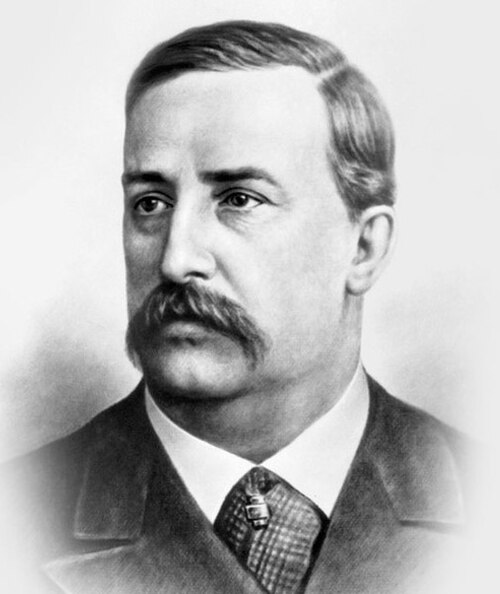
\includegraphics[width=\linewidth]{images/book3/borodin.jpg}
\end{minipage}\hspace{0.02\linewidth}%
\begin{minipage}[t]{0.18\linewidth}
\vspace{0pt}
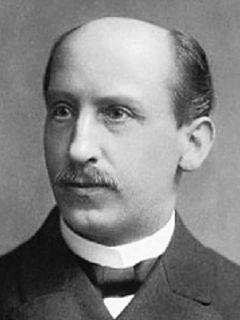
\includegraphics[width=\linewidth]{images/book3/claisen.jpg}
\end{minipage}\hfill
\begin{minipage}[t]{0.58\linewidth}
\vspace{0pt}
羟醛反应于 1872 年由夏尔·阿道夫·伍尔茨
与亚历山大·鲍罗丁独立描述。鲍罗丁是圣彼得堡的化学家，今天更为人知的身份是歌剧 《伊戈尔王》 的作曲家。
路德维希·克莱森于 1887 年把羰基化合物的缩合推广到酯类。（肖像：鲍罗丁，
作者不详，公有领域；克莱森，Veronica.villagrasa 作，CC BY-SA 4.0；维基共享资源。）
\end{minipage}
\end{history}

\begin{safety}{\ghs[5mm]{GHS02}\,\ghs[5mm]{GHS05}\,\ghs[5mm]{GHS07}}
乙醇钠和二异丙基氨基锂具有腐蚀性，且遇水反应；LDA 溶液
易燃，需在惰性气体中操作。苯甲醛和丙酮有害且易燃。
% ledger: ghs:NaOEt, ghs:LDA, ghs:benzaldehyde, ghs:acetone
\end{safety}

\section{练习}

\begin{exercise}[$\star$]\label{exo:b2:enolates-aldol:1}
画出丁酮和环己酮的烯醇式互变异构体。
\end{exercise}

\begin{exercise}[$\star$]\label{exo:b2:enolates-aldol:2}
按各自最酸性的 \ce{C-H} 的酸性强弱排序：丙酮、戊烷-2,4-二酮、3-氧代丁酸乙酯、
乙烷。
\end{exercise}

\begin{exercise}[$\star$]\label{exo:b2:enolates-aldol:3}
写出乙醛与氢氧化钠反应的羟醛产物和缩合产物。
\end{exercise}

\begin{exercise}[$\star$]\label{exo:b2:enolates-aldol:4}
写出由丙二酸酯合成己酸的路线：需要哪种卤代烷？
\end{exercise}

\begin{exercise}[$\star\star$]\label{exo:b2:enolates-aldol:5}
画出 2-甲基环己酮的动力学与热力学烯醇负离子，并说明各自
所需的条件。
\end{exercise}

\begin{exercise}[$\star\star$]\label{exo:b2:enolates-aldol:6}
求苯甲醛与丙酮（各一当量）的交叉羟醛缩合产物，
并解释苯甲醛为何不能自身缩合。
\end{exercise}

\begin{exercise}[$\star\star$]\label{exo:b2:enolates-aldol:7}
己烷-2,5-二酮在碱性条件下发生分子内羟醛缩合，会生成哪种环？请说明
在可能生成的环之间如何选择。
\end{exercise}

\begin{exercise}[$\star\star$]\label{exo:b2:enolates-aldol:8}
写出乙酸乙酯的克莱森缩合反应及其经酸性后处理后的产物。
\end{exercise}

\begin{exercise}[$\star\star$]\label{exo:b2:enolates-aldol:9}
下列哪些物质能给出阳性碘仿反应：丙酮、戊-3-酮、乙醛、苯乙酮？
\end{exercise}

\begin{exercise}[$\star\star\star$]\label{exo:b2:enolates-aldol:10}
写出己二酸二乙酯的狄克曼环化反应，并给出产物的环大小。
\end{exercise}

\begin{exercise}[$\star\star\star$]\label{exo:b2:enolates-aldol:11}
(\textit{R})-3-甲基戊-2-酮在稀氢氧化钠中会失去旋光性，而
(\textit{R})-4-甲基己-2-酮则不会。请解释。
\end{exercise}

\begin{exercise}[$\star\star\star$]\label{exo:b2:enolates-aldol:12}
设计一条路线合成 1,5-二苯基戊-1,4-二烯-3-酮，再合成带有两个不同芳基的二烯酮，
并说明第二步为何更困难。
\end{exercise}

\section{周末问题：二亚苄基丙酮}

\begin{problem}[{周末问题——丙酮的烯醇负离子与苯甲醛的作用、两步羟醛缩合、
共轭产物，以及一次制备的化学计量与产率}]
\label{pb:b2:enolates-aldol:1}
制备（练习数据）：将 \qty{2.1}{mL} 苯甲醛与 \qty{0.75}{mL} 丙酮搅拌
混合于乙醇中，加入氢氧化钠水溶液，析出黄色晶体 1,5-二苯基戊-1,4-二烯-3-酮
（二亚苄基丙酮），产率 75~\%。密度（\unit{g/cm^3}）：苯甲醛 1.045，丙酮 0.7845。
摩尔质量（\unit{g/mol}）：C 12.011，H 1.008，O 15.999。
% ledger: rho:benzaldehyde, rho:acetone, aw:C, aw:H, aw:O, ghs:dibenzalacetone

\medskip
\noindent\textbf{第一部分——反应物。}
\begin{enumerate}
  \item 哪种反应物含有 $\alpha$ 氢？有几个？
  \item 画出丙酮的烯醇负离子。
  \item 为什么苯甲醛不能形成烯醇负离子？
  \item 为什么丙酮与苯甲醛反应，而不与自身反应？
  \item 为什么醛比酮是更好的亲电试剂？
  \item 为什么这里氢氧化物就足以作为碱？
\end{enumerate}

\medskip
\noindent\textbf{第二部分——机理。}
\begin{enumerate}[resume]
  \item 写出烯醇负离子对苯甲醛的加成反应。
  \item 写出生成的羟醛的脱水反应。
  \item 为什么这里的脱水反应容易进行？
  \item 为什么该反应还能发生第二次？
  \item 写出总反应方程式。
  \item 在本制备中，是什么使反应进行完全？
\end{enumerate}

\medskip
\noindent\textbf{第三部分——产物。}
\begin{enumerate}[resume]
  \item 二苄叉丙酮中有几个 \ce{C=C} 双键？主要是哪种构型？
  \item 为什么 (\textit{E},\textit{E}) 异构体更有利？
  \item 数一数共轭 $\pi$ 键的个数。
  \item 为什么该化合物呈黄色，而其反应物均为无色？
  \item 二苄叉丙酮有手性吗？
\end{enumerate}

\medskip
\noindent\textbf{第四部分——化学计量与产率。}
\begin{enumerate}[resume]
  \item 计算苯甲醛、丙酮和二苄叉丙酮的摩尔质量。
  \item 计算两种反应物的物质的量。
  \item 哪种反应物是限量试剂？
  \item 计算产物的理论质量。
  \item 为什么略微过量的苯甲醛比过量的丙酮更好？
  \item 丙酮过量会得到什么？
  \item 求产率为 75~\% 时所得二苄叉丙酮的质量。
\end{enumerate}
\end{problem}
